\section{Atividades}

\subsection{Estabelecer Tema de Investimento}

  \textbf{Descrição}: Essa atividade consiste na definição do tema de investimento a partir do \textit{Workshop} de Requisitos realizado.\\

  \textbf{Tarefas}:

  \begin{itemize}
   \item \indent \textit{Fazer Workshop de Requisitos}: Reunião com o cliente e o time para levantar requisitos de mais alto nível. Consiste
   em uma técnica de elicitação definida no Capítulo \ref{tecnicas}.

   \item \indent \textit{Validar Tema de Investimento}: Escrever o tema de investimento e confirmar com o cliente se
   o Tema de Investimento estabelecido está correto.
  \end{itemize}

  \textbf{Participantes}: \textit{Product Manager}, \textit{Scrum Master}, Time \\

  \textbf{Entradas}: Modelo de negócio \\

  \textbf{Saídas}: Anotações do \textit{Workshop} \\

\subsection{Levantar Épicos}
  \textbf{Descrição}: Essa atividade consiste no levantamento dos épicos com o \textit{Product Manager} através do  \textit{Workshop} de Requisitos. \\

  \textbf{Tarefas}:

  \begin{itemize}
   \item \indent \textit{Fazer Workshop de Requisitos}: Reunião com o cliente e o time para levantar requisitos de mais alto nível. Consiste
   em uma técnica de elicitação definida no Capítulo \ref{tecnicas}.

   \item \indent \textit{Escrever Épicos}: A partir das anotações feitas no \textit{Workshop},
   escrever os épicos no \textit{Backlog} do Programa.

  \end{itemize}

  \textbf{Participantes}: \textit{Product Manager}, \textit{Scrum Master}, Time \\

  \textbf{Entradas}: Anotações do \textit{Workshop} \\

  \textbf{Saídas}: \textit{Backlog} do Programa \\

\subsection{Fazer reunião de validação dos épicos}
  \textbf{Descrição}: Essa atividade consiste na apresentação dos épicos especificados para o \textit{Product Manager}, de modo a validar se os épicos
  especificados estão corretos e correspondem ao esperado. \\

  \textbf{Tarefas}:

  \begin{itemize}
    \item \indent \textit{Validar Épicos}: Confirmar em reunião com o cliente se os épicos estabelecidos estão corretos.

   \item \indent \textit{Escrever Épicos}: Se houver alguma mudança solicitada pelo cliente, escrever os épicos
   refinados no \textit{Backlog} do Programa.
  \end{itemize}

  \textbf{Participantes}: \textit{Product Manager}, \textit{Scrum Master}, Time \\

  \textbf{Entradas}: \textit{Backlog} do Programa \\

  \textbf{Saídas}:  Não se aplica\\

\subsection{Levantar \textit{Features}}
\textbf{Descrição}: Essa atividade consiste em listar as \textit{Features}, a partir dos épicos ,
que são as tarefas ou os “serviços” que o sistema deve fornecer para atender as necessidades das partes interessadas.
Deve-se observar se as \textit{features} condizem com ou traduzem de forma clara os Épicos
definidos previamente, e se através delas é possível escrever as Histórias de Usuário.\\

\textbf{Tarefas}:

  \begin{itemize}
   \item \indent \textit{Listagem de Features}:  Listar Features a partir dos Épicos de Portfólio ou a partir de outras Features.

   \item \indent \textit{Adição e Edição de Features}: Adicionar novas Features ou modificar as Features já levantas de acordo com as mudanças sugeridas na Reunião de Validação.

   \item \indent \textit{Manter Rastreabilidade}: Registrar na ferramenta de qual épico é cada \textit{Feature}.
   \end{itemize}

\textbf{Participantes}: \textit{Product Manager}, \textit{Scrum Master}, Time \\

\textbf{Entradas}: \textit{Backlog} do Programa (épicos) \\

\textbf{Saídas}:   \textit{Backlog} do Programa \\

\subsection{Fazer reunião de validação das \textit{features}}
  \textbf{Descrição}: Essa atividade consiste na apresentação das \textit{features} especificadas para o \textit{Product Manager}, de modo a validar se
  estão corretos e correspondem ao esperado.  \\

  \textbf{Tarefas}:
  \begin{itemize}
   \item \indent \textit{Listagem de Features}: Listar as Features elicitadas e detalhadas até o momento;

   \item \indent \textit{Comparação Features-Épicos}: Comparar as Features e os Épicos, validando se as Features expressam as iniciativas contidas nos Épicos;

   \item \indent \textit{Corrigir Possíveis Falhas}: Identificar equívocos no levantamento ou elicitação das Features e propor mudanças.
  \end{itemize}

  \textbf{Participantes}: \textit{Product Manager}, \textit{Scrum Master}, Time \\

  \textbf{Entradas}: \textit{Backlog} do Programa \\

  \textbf{Saídas}:  Não se aplica\\

\subsection{Identificar Requisitos Não Funcionais}
  \textbf{Descrição}: Nesta atividade são identificados e descritos os requisitos não funcionais do sistema e são armazenados no Backlog do Programa.  \\

  \textbf{Tarefas}:
  \begin{itemize}
   \item \indent \textit{Identificação de Requisitos não Funcionais}: Identificar e descrever os requisitos não funcionais

   \item \indent \textit{Armazenamento no Backlog}: Armazenar no Backlog do Programa
  \end{itemize}

  \textbf{Participantes}: \textit{Product Manager}, \textit{Scrum Master}, Time \\

  \textbf{Entradas}:  Não se aplica\\

  \textbf{Saídas}:  \textit{Backlog} do Programa\\

\subsection{Construir Visão}
  \textbf{Descrição}: Nesta atividade, deve-se compilar as \textit{Features}, com os requisitos não funcionais, incluindo elementos
  regulatórios ou outros padrões de conformidade, e qualquer restrição de design. A partir disso, é possível descrever um panorama da solução a
  ser desenvolvida, refletindo as necessidades das partes interessadas e os recursos propostos para atender essas necessidades. \\

  \textbf{Tarefas}:
  \begin{itemize}
   \item \indent \textit{Reunir Artefatos}: Reunir Features, Requisitos não Funcionais, restrições e padrões.

   \item \indent \textit{Sintetizar e Integrar}: Sintetizar todas as entradas, integrando-as em uma visão holística (global) e coesa do projeto.

   \item \indent \textit{Priorizar Features}: Priorizar as Features no Backlog do Programa.

   \item \indent \textit{Planejamento do RoadMap}: Planejar o RoadMap de entregas das Features.
  \end{itemize}

  \textbf{Participantes}: \textit{Product Manager}, \textit{Scrum Master}, Time \\

  \textbf{Entradas}: \textit{Backlog} do Programa, Requisitos Não funcionais \\

  \textbf{Saídas}:  Visão\\

\subsection{Construir \textit{Roadmap}}
  \textbf{Descrição}: A partir da Visão, deve-se elaborar uma espécie de roteiro, que situa e comunica a equipe e o programa em relação ao
  alinhamento dos objetivos de negócios, e fornece visibilidade das entregas ao longo de um cronograma de curto prazo.
  Esse roteiro divide as \textit{features} nas Releases. \\

  \textbf{Tarefas}:
  \begin{itemize}
   \item \indent \textit{Reunir Documento de Visão}: Reunir o documento de visão

   \item \indent \textit{Definir Prioridades}: Priorizar Features no Backlog do programa.

   \item \indent \textit{Alocamento de Features}: Alocar Features em Releases.

   \item \indent \textit{Escrever}: Escrever histórias
  \end{itemize}

  \textbf{Participantes}: \textit{Product Manager}, \textit{Scrum Master}, Time \\

  \textbf{Entradas}: Visão \\

  \textbf{Saídas}:  \textit{Roadmap}\\

\begin{figure}[!htb]
\centering
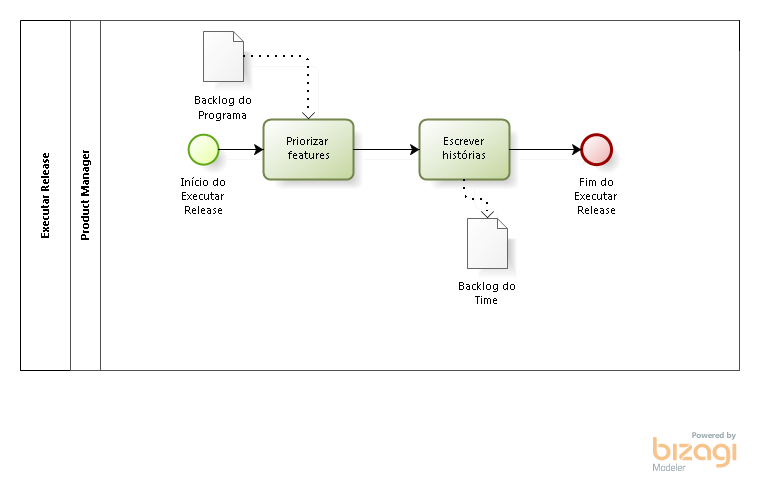
\includegraphics[scale=0.7]{figuras/release.png}
\caption{Subprocesso Executar Release}
\label{fig:release}
\end{figure}

A partir do Subprocesso da Figura \ref{fig:release} o processo contém as seguintes atividades.

\subsection{Priorizar \textit{features}}
  \textbf{Descrição}: Essa atividade consiste na priorização das \textit{features} para a Release. \\

  \textbf{Tarefas}:
  \begin{itemize}
   \item \indent \textit{Reunir Features}: Reunir features envolvidas no processo;

   \item \indent \textit{Estudar as Features}: Estudar as features para melhor entendimento de cada uma;

   \item \indent \textit{Definir Indicador de Complexidade}: Definir um identificador para saber quais demandam mais trabalho (horas de serviço);

   \item \indent \textit{Ordenar}: A partir dos resultados obtidos via análise, ordenar das que mostraram maiores métricas de esforço, até as menores, de modo que as mais difíceis sejam executadas o quanto antes.
  \end{itemize}

  \textbf{Participantes}: \textit{Product Manager}, \textit{Scrum Master}, Time\\

  \textbf{Entradas}: \textit{Backlog} do Programa \\

  \textbf{Saídas}:  Não se aplica\\

\subsection{Escrever histórias}
  \textbf{Descrição}: Essa atividade consiste na escrita das histórias em um nível macro, derivadas das \textit{features}, para composição do \textit{Backlog} do Time. \\

  \textbf{Tarefas}:
  \begin{itemize}
   \item \indent \textit{Identificar}: Identificar features;

   \item \indent \textit{Analisar}: Analisar o nível de prioridade das features;

   \item \indent \textit{Alocar}: Alocar features nas sprints;

   \item \indent \textit{Instruir}: Auxílio do Scrum Master ao Product Manager a fim de ensinamento; de técnicas de escritas de histórias de usuário;

   \item \indent \textit{Escrita}: Escrever histórias;

   \item \indent \textit{Armazenamento}: Armazenar histórias no Backlog do time.
  \end{itemize}

  \textbf{Participantes}: \textit{Product Manager}, \textit{Scrum Master}, Time\\

  \textbf{Entradas}: \textit{Backlog} do Programa \\

  \textbf{Saídas}:   \textit{Backlog} do Time \\

\begin{figure}[!htb]
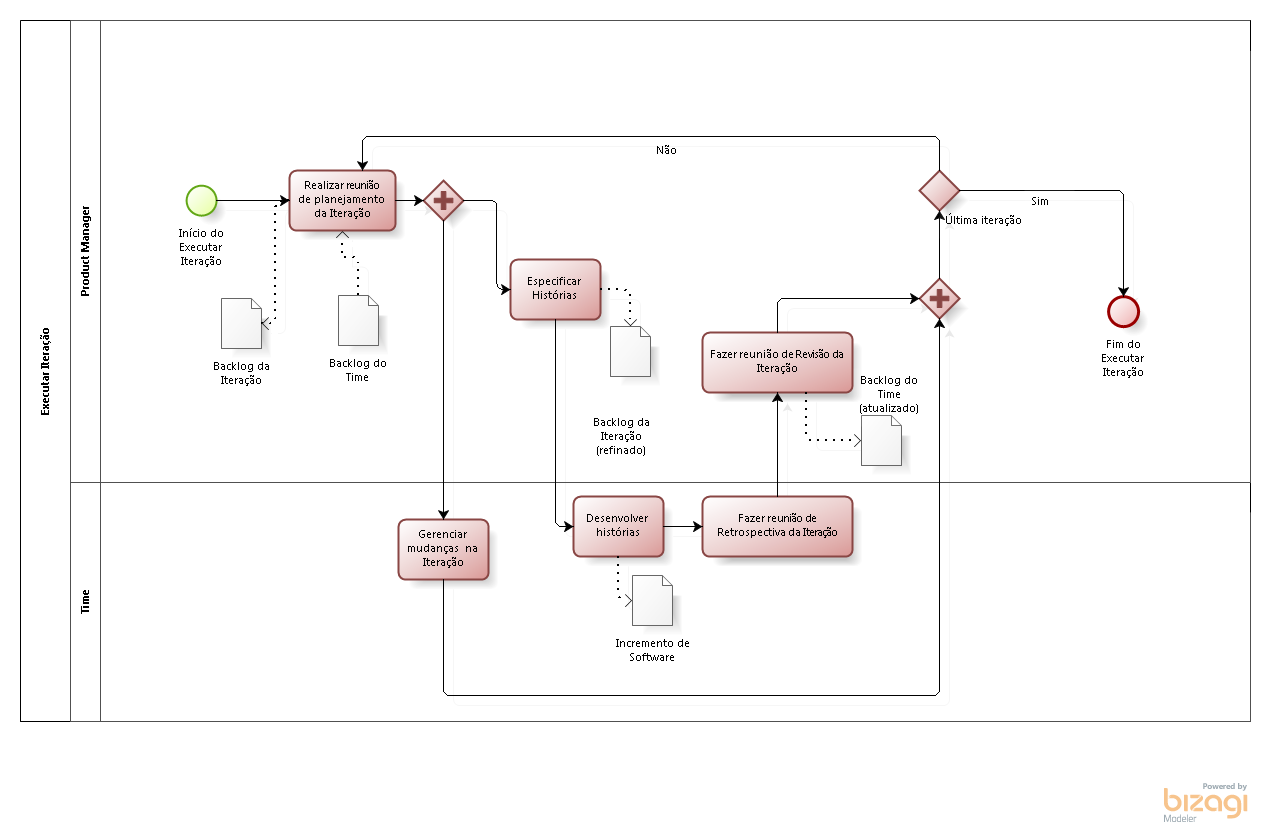
\includegraphics[scale=0.5]{figuras/iteracao.png}
\caption{Suprocesso Executar Iteração}
\label{fig:iteracao}
\end{figure}

A partir do Subprocesso da Figura \ref{fig:iteracao} o processo contém as seguintes atividades.

\subsection{Realizar reunião de planejamento da Iteração}
  \textbf{Descrição}: Essa atividade consiste no planejamento da iteração através da alocação das histórias definidas no \textit{Backlog} do Time para o \textit{Backlog} da Sprint. \\

  \textbf{Tarefas}:
  \begin{itemize}
   \item \indent \textit{Alocação das Histórias}: Alocação das histórias no Backlog da Sprint

   \item \indent \textit{Armazenamento de Artefatos}: Armazenar no Backlog de Iteração
  \end{itemize}

  \textbf{Participantes}: \textit{Product Manager}, \textit{Scrum Master}, Time\\

  \textbf{Entradas}: \textit{Backlog} do Time \\

  \textbf{Saídas}:  \textit{Backlog} da Iteração\\

\subsection{Especificar histórias}
  \textbf{Descrição}: Essa atividade consiste na escrita mais detalhada das histórias que irão compor a
iteração. \\

  \textbf{Tarefas}:
  \begin{itemize}
   \item \indent \textit{Detalhamento das Histórias}: Detalhar histórias da iteração

   \item \indent \textit{Armazenamento de Artefatos}: Armazenar no Backlog de Iteração

   \item \indent \textit{Atualizar}: Atualizar Backlog do Time
  \end{itemize}

  \textbf{Participantes}: \textit{Product Manager}, \textit{Scrum Master}, Time\\

  \textbf{Entradas}: \textit{Backlog} da Iteração \\

  \textbf{Saídas}:   \textit{Backlog} da Iteração (refinado)\\

\subsection{Desenvolver histórias}
  \textbf{Descrição}: Essa atividade consiste no desenvolvimento e teste das histórias contidas no Backlog da Iteração. Tem uma duração de 1 semana. \\

  \textbf{Tarefas}:

  \begin{itemize}
    \item \indent \textit{Desenvolver Histórias}: Implementar as histórias contidas no \textit{Backlog} da Iteração.

   \item \indent \textit{Testar Histórias}: Realizar testes unitários do código implementado na iteração e testes funcionais
   com base nos testes de aceitação.
  \end{itemize}

  \textbf{Participantes}: Time\\

  \textbf{Entradas}: \textit{Backlog} da Iteração \\

  \textbf{Saídas}:   Incremento de Software\\

\subsection{Fazer reunião de revisão e retrospectiva da Iteração}
  \textbf{Descrição}: Essa atividade consiste na validação das histórias implementadas através da execução dos testes de aceitação. \\

  \textbf{Tarefas}:
  \begin{itemize}
   \item \indent \textit{Analise de Artefatos}: Analisar artefatos gerados na iteração;

   \item \indent \textit{Avaliar Pontos Positivos}: Definir pontos que ocorreram bem;

   \item \indent \textit{Definir Pontos de Melhoria}: Definir pontos que necessitam de melhoria;

   \item \indent \textit{Definir Novas Metas}: Definir novas metas de melhoria a serem alcançadas na nova sprint.
  \end{itemize}

  \textbf{Participantes}: \textit{Product Manager}, Time\\

  \textbf{Entradas}: Incremento de Software \\

  \textbf{Saídas}:   \textit{Backlog} da Iteração (atualizado)\\
